\section{Experimental Results}
\label{sec:results}

Unless stated otherwise, results refer to the 810 held-out configurations (90 query vectors $\times$ 9 levels).

\subsection{Overall Performance}
Table~\ref{tab:overall} summarizes the held-out results. Of the four baselines, only exact search (B1) and iterative
HNSW (B2-iter) meet the quality targets. Single-pass HNSW (B2-plain) and PostgreSQL's default plan choice (B3) are
the fastest in raw latency but return incomplete answers for 60.4\% and 27.0\% of the queries. Among the methods that
meet both targets, P1 has the lowest p50, p95 and mean latency. Its p50 of 1.332\,ms (95\% CI 1.254--1.417) is 51\%
below that of B2-iter (2.716\,ms), the best qualifying baseline at the median. Its p95 of 3.297\,ms (2.956--3.540) is
80\% below that of B1 (16.344\,ms), the best qualifying baseline in the tail. Both paired differences exclude zero:
$[-1.687,-1.265]$\,ms and $[-13.386,-12.806]$\,ms. B1's recall is 0.99988 rather than 1 because of a single
numerical near-tie at rank 10; its tie-tolerant recall is 1.

\begin{table}[t]
\caption{Held-out results (810 configurations). Latency in ms (per-configuration median of five runs);
R@10 is mean strict Recall@10; Q marks methods meeting both quality targets}
\label{tab:overall}
\centering
\footnotesize
\setlength{\tabcolsep}{3.4pt}
\begin{tabular}{@{}lrrrrrc@{}}
\toprule
Method & p50 & p95 & Mean & R@10 & Compl. & Q\\
\midrule
B1 exact        & 4.159 & 16.344 & 6.688 & 1.000 & 100.0\% & $\checkmark$\\
B2-plain        & 1.414 & 1.901  & 1.411 & 0.510 & 39.6\%  & $\times$\\
B2-iter         & 2.716 & 25.758 & 7.049 & 0.968 & 99.5\%  & $\checkmark$\\
B3 planner      & 1.233 & 1.818  & 1.204 & 0.828 & 73.0\%  & $\times$\\
\textbf{P1 router} & \textbf{1.332} & \textbf{3.297} & \textbf{1.511} & \textbf{0.991} & \textbf{100.0\%} & $\checkmark$\\
\midrule
Oracle (floor)$^{a}$ & 1.313 & 3.247 & 1.469 & 0.991 & 100.0\% & --\\
B3+iter$^{b}$   & 1.359 & 5.415  & 1.873 & 0.989 & 100.0\% & $\checkmark$\\
\bottomrule
\multicolumn{7}{@{}p{\columnwidth}@{}}{\scriptsize $^{a}$Per-configuration minimum of B1 and B2-iter in hindsight;
its quality is reported, not enforced. $^{b}$Supplementary: default plan choice with iterative scanning enabled.}
\end{tabular}
\end{table}

\begin{figure*}[t]
\centering
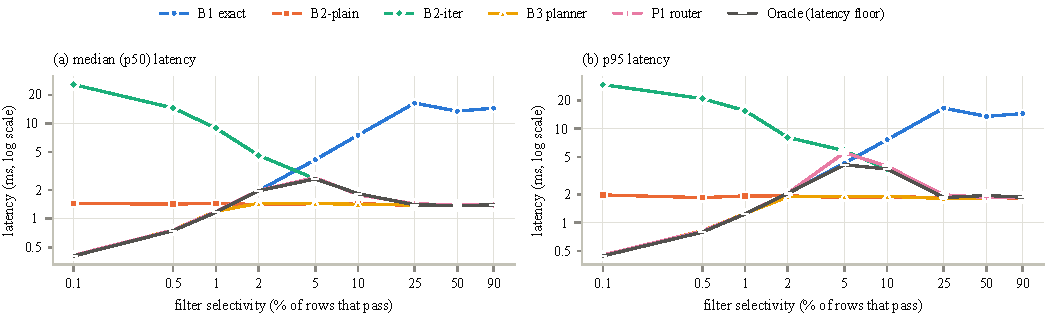
\includegraphics[width=\textwidth]{figures/latency_vs_selectivity.pdf}
\caption{End-to-end latency versus filter selectivity on the held-out split (log--log). B1 and B2-iter cross between
2\% and 5\%; P1 follows the lower envelope of the two arms and nearly coincides with the Oracle latency floor. B2-plain
and B3 are fast but incomplete below 25\% (Fig.~\ref{fig:quality}).}
\label{fig:latency}
\end{figure*}

\subsection{Performance Across Filter Selectivities}
Fig.~\ref{fig:latency} shows the opposite cost trends of the two arms (RQ1). The median latency of B1 grows from
0.41\,ms at 0.1\% to 16.3\,ms at 25\%, because every eligible row is fetched and its 512-dimensional distance
computed. Between 25\% and 50\%, the planner switches B1 from a non-parallel bitmap scan to a parallel sequential scan,
which makes 25\% B1's slowest level (13.4\,ms at 50\%, 14.5\,ms at 90\%). B2-iter shows the reverse trend: 25.5\,ms at
0.1\%, 8.9\,ms at 1\% and about 1.4\,ms from 25\% upwards. Under a selective filter almost every traversed candidate is
discarded, so the iterative scan keeps expanding; at 0.1\% it sometimes exhausts its scan budget before finding ten
qualifying rows (Section~\ref{sec:quality}). The arms cross between 2\% (B1 1.97\,ms vs.\ B2-iter 4.62\,ms) and 5\%
(4.16 vs.\ 2.62\,ms). P1 sends every configuration up to 2\% to B1 and every one from 10\% upwards to B2-iter, so it
tracks the lower envelope. At 5\% it routes 89 of 90 configurations to B2-iter, because the frozen threshold
($T^{*}=4{,}696$ estimated rows) lies just below the typical estimate of about 5{,}000.

\subsection{Retrieval Quality}
\label{sec:quality}
Fig.~\ref{fig:quality} explains why the two fastest baselines fail the targets. B2-plain inspects only
\code{ef\_search=100} candidates, and under a selective filter too few survive: it is never complete at 0.1\%--2\%,
10\% complete at 5\% and 50\% complete at 10\%. B3 uses an exact B-tree plan up to 1\%, but from 2\% upwards
PostgreSQL's planner selects the non-iterative HNSW scan. B3 then inherits B2-plain's incompleteness exactly (0\%
complete and Recall@10 0.217 at 2\%), consistent with the planner behavior reported in~\cite{amanbayev2026filtered}.
Iterative scanning largely restores completeness, but not at the most selective level: at 0.1\%, B2-iter is complete
for 95.6\% of queries with recall 0.844, because the scan budget runs out first. P1 avoids this regime by
construction. Its per-level recall is at least 0.978, and it is complete for every held-out query.

\begin{figure}[t]
\centering
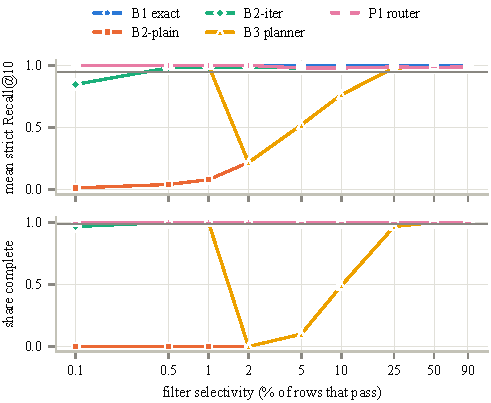
\includegraphics[width=\columnwidth]{figures/quality_vs_selectivity.pdf}
\caption{Mean strict Recall@10 (top) and completeness (bottom) on the held-out split; horizontal lines mark the targets
0.95 and 0.99. P1 coincides with B1 up to 2\% and with B2-iter from 5\%.}
\label{fig:quality}
\end{figure}

\subsection{Selectivity Estimation Accuracy}
Fig.~\ref{fig:estimation} compares the cached \code{pg\_stats} estimates with the actual counts for all 2{,}700
filters. The mean relative error falls from 11.2\% at 0.1\% (about 11 rows) to 4.3\% at 1\%, 1.9\% at 5\% and 0.2\% at
90\%. With 100 equi-depth buckets of about 1\% each, narrower ranges are interpolated within one bucket, and a few narrow
ranges in sparse regions are underestimated tenfold (Fig.~\ref{fig:estimation}a). Our estimator reproduces PostgreSQL's own
planner estimate with a median relative difference of 0.02\% (95th percentile 1.1\%), so the router sees what the
optimizer sees. For routing, only errors near the threshold matter. On both splits, all 0.1\%--2\% estimates (at most
2{,}145 rows) lie far below $T^{*}$ and all 10\%--90\% estimates (at least 9{,}094) far above it. Misestimation
therefore affects routing only at 5\%, whose estimates range from 4{,}105 to 5{,}249 rows.

\begin{figure}[t]
\centering
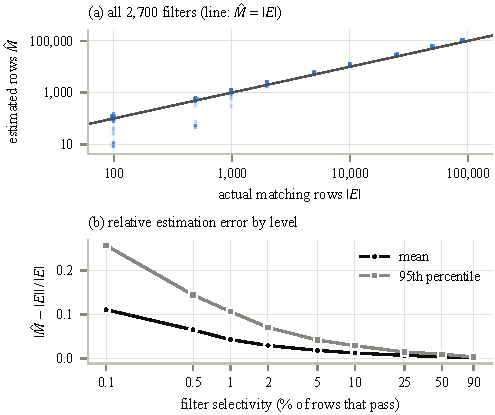
\includegraphics[width=\columnwidth]{figures/estimation.pdf}
\caption{Histogram-based row estimates versus actual matching rows for all 2{,}700 filters (a), and relative error by
selectivity level (b).}
\label{fig:estimation}
\end{figure}

\subsection{Proposed Router versus Baselines}
P1 thus meets all pre-registered criteria on the held-out split (RQ2). Calibration and evaluation agree closely: the
simulated router at $T^{*}$ had a mean of 1.437\,ms, a p95 of 2.876\,ms and a recall of 0.994 on the calibration split
(44.7\% of configurations sent to B1), versus 1.511\,ms, 3.297\,ms and 0.991 measured on the held-out split. This
does not mean that P1 wins at every level. Table~\ref{tab:perlevel} compares P1 with the best
qualifying baseline \emph{at each level}, which is usually the arm P1 itself selects. Under this strict criterion,
P1 is not faster at any level for both statistics. In most cells the difference is a few tens of microseconds and
its paired interval contains zero. Three differences are distinguishable: P1 is 11 and 19\,$\mu$s slower than B1 at
the 0.5\% and 1\% medians, where both run the identical exact plan, and 1.26\,ms slower than B1 at the 5\% p95
(Section~\ref{sec:negative}).

\begin{table*}[t]
\caption{P1 versus the best qualifying baseline at each level (held-out). Latency in ms; $\Delta=$ P1 $-$ best with
95\% paired bootstrap interval; $^{\dagger}$: interval excludes zero. Routed: configurations sent to B1 by P1 / by the
Oracle (of 90)}
\label{tab:perlevel}
\centering
\footnotesize
\setlength{\tabcolsep}{4.2pt}
\begin{tabular}{@{}rclrrlclrrl@{}}
\toprule
& Routed & \multicolumn{4}{c}{p50} & & \multicolumn{4}{c}{p95}\\
\cmidrule(lr){3-6}\cmidrule(l){8-11}
Level & to B1 & Best & best & P1 & $\Delta$ [95\% CI] & & Best & best & P1 & $\Delta$ [95\% CI]\\
\midrule
0.1\% & 90/90 & B1      & 0.407 & 0.414 & $+0.006$ $[-0.001,\,0.015]$ & & B1 & 0.444 & 0.454 & $+0.009$ $[-0.013,\,0.032]$\\
0.5\% & 90/90 & B1      & 0.749 & 0.760 & $+0.011$ $[0.001,\,0.019]^{\dagger}$ & & B1 & 0.795 & 0.817 & $+0.022$ $[-0.009,\,0.034]$\\
1\%   & 90/90 & B1      & 1.169 & 1.188 & $+0.019$ $[0.005,\,0.031]^{\dagger}$ & & B1 & 1.243 & 1.242 & $-0.000$ $[-0.022,\,0.021]$\\
2\%   & 90/89 & B1      & 1.967 & 1.979 & $+0.011$ $[-0.010,\,0.025]$ & & B1 & 2.055 & 2.066 & $+0.011$ $[-0.040,\,0.052]$\\
5\%   & 1/13  & B2-iter & 2.622 & 2.702 & $+0.080$ $[-0.055,\,0.429]$ & & B1 & 4.314 & 5.575 & $+1.261$ $[0.155,\,3.006]^{\dagger}$\\
10\%  & 0/0   & B2-iter & 1.834 & 1.785 & $-0.049$ $[-0.105,\,0.114]$ & & B2-iter & 3.730 & 3.994 & $+0.264$ $[-0.197,\,0.498]$\\
25\%  & 0/0   & B2-iter & 1.401 & 1.434 & $+0.032$ $[-0.075,\,0.090]$ & & B2-iter & 1.854 & 1.987 & $+0.132$ $[-0.035,\,0.332]$\\
50\%  & 0/0   & B2-iter & 1.376 & 1.399 & $+0.023$ $[-0.038,\,0.073]$ & & B3 & 1.842 & 1.860 & $+0.018$ $[-0.073,\,0.138]$\\
90\%  & 0/0   & B2-plain& 1.377 & 1.392 & $+0.014$ $[-0.073,\,0.057]$ & & B2-plain & 1.823 & 1.871 & $+0.048$ $[-0.090,\,0.159]$\\
\bottomrule
\end{tabular}
\end{table*}

\subsection{Oracle Comparison}
Relative to the best qualifying baseline, P1 captures $\Gamma=98.7\%$ of the Oracle's latency reduction at the median
(B2-iter 2.716, P1 1.332, Oracle 1.313\,ms), 99.6\% at p95 (B1 16.344, P1 3.297, Oracle 3.247\,ms) and 99.2\% for the
mean (B1 6.688, P1 1.511, Oracle 1.469\,ms). Its routing agrees with the Oracle on 98.1\% of configurations; 14 of the
15 disagreements occur at 5\%. The Oracle knows both arms' latencies in hindsight, pays no overhead and enforces no
quality constraint; its recall (0.991) and completeness (100\%) merely happen to be high here. Per level, the ratio is
mostly undefined because the Oracle is not faster than the best baseline (both are B1 up to 1\%).

\subsection{Additional Findings and Negative Results}
\label{sec:negative}
\textbf{Iterative scanning with the default planner.} Enabling iterative scanning and letting PostgreSQL choose the plan
(B3+iter) meets the quality targets, but its p95 is 64\% and its mean 24\% higher than P1's (Table~\ref{tab:overall}).
The plan choice is identical to B3's, because iterative scanning changes execution, not costing. From 2\% upwards the
planner selects HNSW where iterative HNSW is slower than exact search: at 2\%, B3+iter takes 4.66\,ms at the median
versus 1.98\,ms for P1. Iterative scanning repairs completeness but leaves the crossover in the wrong place.

\textbf{The 5\% level and the limits of one threshold.} The calibration objective is nearly flat: every feasible $T$
between 2{,}129 and 4{,}842 estimated rows is within 1\% of the minimum mean latency (Fig.~\ref{fig:calibration}).
The pre-registered rule picked the minimizer $T^{*}=4{,}696$, which lies inside the 5\% level's range of estimates, so
P1 sent 89 of 90 of those configurations to B2-iter. At 5\%, B2-iter is faster at the median (2.62 vs.\ 4.16\,ms for
B1) but has a heavier tail (p95 5.85 vs.\ 4.31\,ms), and the Oracle would have sent 13 configurations to B1. Moving
$T$ cannot remove this p95 loss: a lower $T$ routes the same configurations to B2-iter, and a higher $T$ sends the
whole level to B1, raising its median to about 4.2\,ms. Near the crossover the faster arm depends on the query vector
and filter position, which a cardinality threshold cannot observe. $T^{*}$ was not re-tuned after the held-out run.

\begin{figure}[t]
\centering
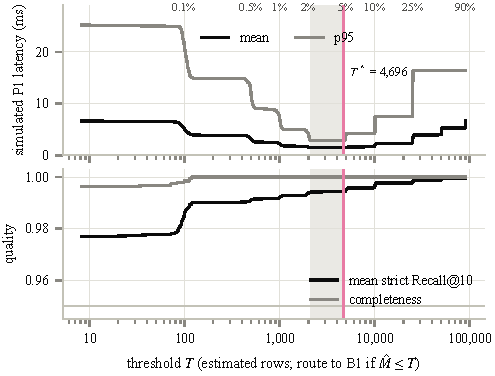
\includegraphics[width=\columnwidth]{figures/calibration_curve.pdf}
\caption{Threshold calibration on the calibration split: simulated P1 latency (top) and quality (bottom) versus $T$.
The shaded band holds every feasible $T$ within 1\% of the minimum mean latency; labels mark each level's median
estimate; the vertical line is the frozen $T^{*}$.}
\label{fig:calibration}
\end{figure}

\textbf{Routing overhead.} An estimate plus decision takes 0.6\,$\mu$s in a tight loop. Measured live between database
round trips it takes 9.6\,$\mu$s at the median (14.9\,$\mu$s p95), and P1 is 8.4\,$\mu$s slower than its chosen arm.
This cost is negligible for millisecond queries but visible at the most selective levels, where P1 and B1 run the same
sub-millisecond plan (Table~\ref{tab:perlevel}).

\textbf{HNSW sensitivity (calibration split).} At the 90\% level, setting \code{ef\_search} to 40, 100 and 200 gives medians of 0.83, 1.29 and 1.92\,ms at recall 0.986, 0.996 and 0.999, but none fixes completeness at 0.1\% (96.7\%--97.1\%). A \code{max\_scan\_tuples} of 100{,}000 lifts it to 98.6\% at a p95 of 37.6 instead of 30.8\,ms, and \code{strict\_order} lowers overall recall from 0.977 to 0.968. These settings shift the crossover but do not remove it.
